\chapter{The Silence}
\label{ch:13}



\begin{center}
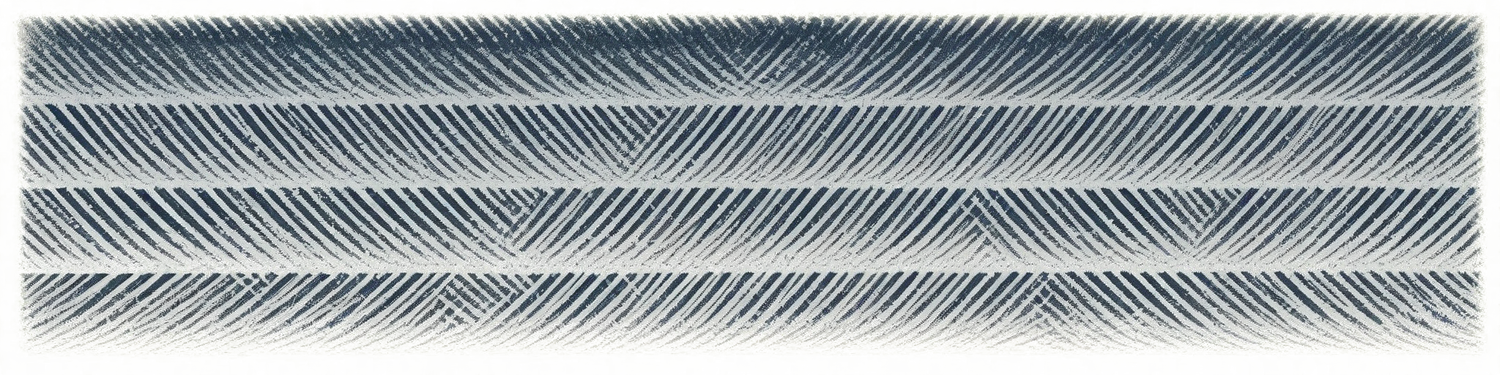
\includegraphics[width=\textwidth]{images/chapterImages/genesis_sketch_00090_.png}
\end{center}

The wrongstar filled a third of the sky now. Not a point. Not a disk. A presence. Massive enough that its shape was visible—irregular, tumbling slowly, the surface showing variations in brightness where different materials reflected differently. The tail streamed behind it like fire, stretching halfway across the visible sky.

45 rotations remaining.

The heat was constant. Day and night had lost meaning. There was only bright and brighter. Hot and hotter. The temperature had risen enough that many plants had stopped functioning. Forests showed signs of stress—leaves curling, trees dropping foliage early, whole sections of vegetation beginning to die from the sustained thermal assault.

Animals fled in random directions. Migrations that made no evolutionary sense. Instinct firing desperately in the face of threat too large to comprehend. Most would die from the disruption alone, before the impact even occurred. The ecosystem was already collapsing under the strain of approaching catastrophe.

But the dinosaurs remained calm. They had calculated this. Expected this. Knew that the pre-impact effects would be devastating. Knew that it didn't matter because the impact itself would be so much worse that these preliminary deaths were rounding errors in the final total.

They moved toward their chosen places. Gathered with intention. Prepared for ending.

\scenebreak

Aurelia left her territory for the final time. The pattern would remain where it was. Already showing erosion from the violent weather. Stones displaced by wind. Sections disrupted. The encoding degrading as she had always known it would.

It had served its purpose. Had existed long enough for verification. For contribution to collective understanding. For demonstrating that the mathematics was complete. What happened to it now was irrelevant.

She traveled toward the northern plateau—a high, exposed location far from the predicted impact site but with clear lines of sight in all directions. A place where watching would be unobstructed. Where the final calculations could be confirmed through direct observation. Where consciousness could witness its own ending with full awareness of what was ending and why.

Others moved along parallel paths. She could sense them without seeing them. The feeling of presence that came from shared direction, shared purpose. They were all converging on gathering points. Not randomly. Not instinctively. Through calculation that had identified optimal witness locations given impact trajectory and shockwave propagation patterns.

The journey took four rotations. She didn't hurry. Didn't conserve energy. There was no need for conservation anymore. No future that required physical reserves. Just the present moment extending forward for 45 more rotations until it terminated.

When she arrived at the northern plateau, dozens were already there. More appeared as she watched—individuals and small family groups emerging from different directions, all converging on this calculated point.

The massive long-necks stood at the plateau's edge, their huge bodies somehow appearing fragile against the scale of sky-filling wrongstar. The swift runners clustered together, their speed advantage meaningless now. The armored ones had shed their defensive postures—no threat remained that armor could stop.

And everywhere, the small ones. The thinkers. The calculators. Hundreds of them. Standing in loose formation that somehow organized itself without coordination. Each individual finding a position that felt correct. That fit the mathematics of optimal witness configuration.

Aurelia found her position. It was waiting for her—not marked, not designated, just recognized as correct when she arrived at it. She settled into stance and looked at the sky.

Around the plateau, other gathering points were similarly occupied. She couldn't see them but knew they existed. The calculations had identified seventeen optimal witness locations given global distribution and viewing angle requirements. All seventeen would be occupied. All seventeen would observe the same event from different perspectives. Final data collection. Last confirmation that the trajectory calculations were correct.

Not that it mattered if they were correct. There was no time left for adjustments. No possibility of evasion. The wrongstar would arrive where calculations said it would arrive. Would impact with the energy calculations predicted. Would reshape the planet according to mathematical certainty.

But they would watch anyway. Would confirm the calculations through observation. Would witness the accuracy of their predictions even as those predictions manifested as extinction.

Because that's what consciousness did. Observed. Calculated. Understood until understanding was no longer possible.

\scenebreak

The Builder arrived at the plateau on the third day of gathering. Aurelia recognized him immediately—he had changed since she'd last seen him years ago, scarred and aged by the intensity of his work. But his posture was unmistakable. His movement patterns. The particular quality of stillness he achieved.

He found his position and settled. They were perhaps fifty body lengths apart. Close enough to acknowledge each other's presence. Far enough to maintain individual observational integrity.

They had never directly interacted. Had never shared calculations through anything but the patterns they created independently. But they had worked the same problem. Had arrived at the same solutions. Had encoded their understanding in complementary ways that together formed complete picture.

Acknowledgment passed between them without signal. Just recognition. Just presence. Just the understanding that they had both contributed what they could contribute and now would both witness what that contribution led to.

The Carver never arrived—she had died seasons ago, her work complete. But two of her protégés were present. Young ones who had learned her cliff-carving techniques. Who had added their own sections to the genetic encoding she had begun. Her understanding persisted through them. Her contribution continued through their extensions of her work.

That was sufficient. That was the only form of persistence available to consciousness. Through the work that outlived the worker. Through the knowledge that propagated beyond the knower. Through the calculations that remained valid independent of who had calculated them.

\scenebreak

More arrived. The gathering swelled to hundreds, then thousands. Not every dinosaur on the continent—most had chosen locations closer to their home territories, places significant to their individual experience. But enough gathered here to create the feeling of collective witness. Of shared observation. Of consciousness recognizing itself in multitude before that multitude dispersed forever.

They stood in silence. Not the silence of absence but the silence of complete understanding. No communication was necessary. All calculations were complete. All knowledge was shared. What remained was waiting.

And watching.

The wrongstar grew daily. Hourly. The tumble of its rotation became visible—brighter patches rotating across its surface, darker regions disappearing and reemerging. The detail increased as distance decreased. Soon individual surface features would be distinguishable. Later, the shape would dominate everything. Fill the entire sky from horizon to horizon.

Then: arrival.

The timeline was absolute. 45 rotations at the gathering's start. Now 42. Now 38. Now 33. The countdown continued with mathematical precision. Each rotation confirmed the calculations. Each observation matched prediction. The trajectory was perfect. The impact was inevitable. The extinction was certain.

And they watched it approach with calm acceptance that might have looked like peace if peace was the right word for understanding your own termination.

\scenebreak

On the twentieth rotation before impact, the Pair arrived.

She hadn't seen them since before the work began. Since before the wrongstar had appeared. They had been separate for years—working in distant territories on their own patterns, their own contributions.

Now they were together again.

They entered the gathering side by side. Moving in perfect synchronization. Steps matched. Breathing aligned. They found a position near the plateau's center and settled together. Not just near each other. Pressed together. Flanks touching. Tails intertwined. Physical contact that was constant and complete.

Aurelia observed this with the detached interest of someone watching mathematics resolve into behavior. They had maintained connection across vast distance through unknown means. Had worked separately while somehow remaining unified. Had calculated independently while arriving at identical conclusions. Now they reunited for the final witness.

They were older now. One of them showed significant age—feathers thinned, movements slow, breathing labored. The other was healthier but not much. They had both pushed themselves to the limit of biological capability during the work years.

They would not survive the impact. Their survival probability calculations were essentially zero. They were too old, too worn, too depleted. The impact winter would kill them within days even if the initial shockwave didn't.

They knew this. The calculations were simple enough that even less sophisticated minds could run them. They knew they were dying soon regardless of what they did.

And they had chosen to die together. Pressed against each other. Unified until the end.

Aurelia watched them and understood something that mathematics couldn't quite capture: the work was necessary, but it wasn't sufficient. The encoding mattered, but it wasn't everything. Connection existed that couldn't be quantified. That persisted despite separation. That manifested as physical proximity in final moments not because proximity increased survival probability but because it provided something else. Something the calculations couldn't incorporate but that consciousness required anyway.

She thought of the other one. The one who had helped with her pattern. Who had brought food. Who had stood with tail almost touching. Who had dispersed years ago into constituent elements and couldn't be here for final witness.

She had marked his location. Had continued his pattern section. Had maintained his contribution. But he wasn't present. Couldn't be present. Matter didn't reassemble once dispersed. Consciousness didn't persist beyond biological function.

The Pair demonstrated an alternative: be together until the end. Maintain physical connection. Let the termination happen while unified.

It was too late for her to achieve that. Her companion had dispersed. This ending she would face alone.

But she had encoded her understanding. Had built his contributions into the pattern. Had ensured his calculations persisted even if his consciousness didn't.

That would have to be sufficient.

\scenebreak

The gathering settled into its final configuration. No new arrivals after the twenty-fifth day. Everyone who would witness from this location had arrived. Everyone who wouldn't had chosen different places.

They stood in their positions and watched the wrongstar grow. Watched the detail resolve. Watched the mathematical predictions manifest as observable reality.

The youngest ones present were adolescents—perhaps twenty of them scattered through the gathering. They stood with family groups mostly, though a few stood alone. Their survival probability was higher than the adults'. Small size. Lower resource requirements. Better ability to hide and wait through the resource-scarce years.

Maybe three would survive. Maybe five. Maybe none. The probability curves were broad at the individual level. At the population level, the mathematics was clearer: young ones as a cohort would survive at higher rates. Some specific young ones would persist. Would carry forward whatever understanding they had achieved. Would maintain the work if they survived to breed, to teach, to contribute.

But which specific young ones would survive? That was unknowable. Random within the probability distribution. Chaos determining specific outcome while statistics determined aggregate results.

Some would live. Most would die. That was the calculation.

And it was sufficient. The work didn't require specific individuals to persist. Just enough individuals to maintain species consciousness. To continue protection of mammal populations. To ensure the encoding persisted through the extinction boundary.

\scenebreak

15 rotations remaining.

The wrongstar's shape was fully visible now. Irregular. Tumbling. Massive beyond comprehension. It filled half the sky and continued growing. The tail stretched beyond the horizon—a river of light and matter streaming behind the approaching mountain.

The heat was killing anything that couldn't shelter. Vegetation was dying across vast swaths of territory. Water sources evaporated. Animals succumbed to thermal stress. The ecosystem collapsed in slow motion as a preview of the sudden collapse that was coming.

But in the protected burrows, the mammals endured. Deep underground, insulated by layers of earth, the tool-users and tree-dwellers and all the selected lineages waited out the thermal assault. They didn't understand what was happening. Didn't know why the world was ending. Just hid and endured because hiding and enduring was what their kind did.

They would emerge after the impact. After the shockwave passed. After the immediate danger resolved. Would find a world transformed. Would face conditions that killed most creatures. Would survive or not survive based on combination of preparation, genetics, and random chance.

But they had the capability. The encoded traits. The selected characteristics that increased their probability of persistence.

Eight percent. Still eight percent. The calculation hadn't changed. Wouldn't change now. Eight percent was what mathematics purchased given the constraints of reality.

Aurelia looked at the gathering. Thousands of her kind standing in witness configuration. The most sophisticated consciousness the planet had yet produced. The deepest calculators. The furthest planners. The minds that could hold evolutionary timelines and probability curves and million-year projects in conscious thought.

All of them about to disperse. All consciousness terminating simultaneously. All that intelligence vanishing in a moment.

But not lost. Not entirely. They had encoded their understanding in flesh. Had built their calculations into the mammal populations. Had created a plan that would unfold without them because they had designed it to unfold without them.

They were not the end. They were the beginning. The first consciousness to recognize the possibility of persistence beyond itself. The first to deliberately encode its gifts for future minds. The first to sacrifice everything for the chance—just the chance—that something might continue.

Eight percent was better than zero.

And zero was what they would achieve if they did nothing.

So they had done something. Had calculated and encoded and prepared and positioned. Had created possibility where none had existed. Had purchased eight percent chance of success through years of desperate effort.

And now they would watch that eight percent possibility begin its long, uncertain resolution across 65 million years.

10 rotations remaining.

The wrongstar dominated everything. The only thing visible. The only thing real. Approaching with implacable patience.

Mathematics made manifest.

Extinction approaching on schedule.

The equation preparing to balance.

